 \documentclass{article}
 \usepackage{graphicx}
 \graphicspath{ {./images/} }
 
 \usepackage{hyperref}
 \hypersetup{
    colorlinks=true,
    linkcolor=blue,
    filecolor=magenta,      
    urlcolor=cyan,
 }

 \usepackage{parskip}
 \usepackage{amsmath}
 
 \begin{document}
 
 \begin{center}
     \Huge\textbf{Homework 9: Sukrit Ganesh}\par
 \end{center}
 
  \noindent\makebox[\linewidth]{\rule{\paperwidth}{0.4pt}}\newline
 
 \begin{center}
      \Large\textbf{Problem 1:} On Fig. 10.23, mark the mean of the dataset, the first principal component, and the second principal component. \par
 \end{center}
 
 
 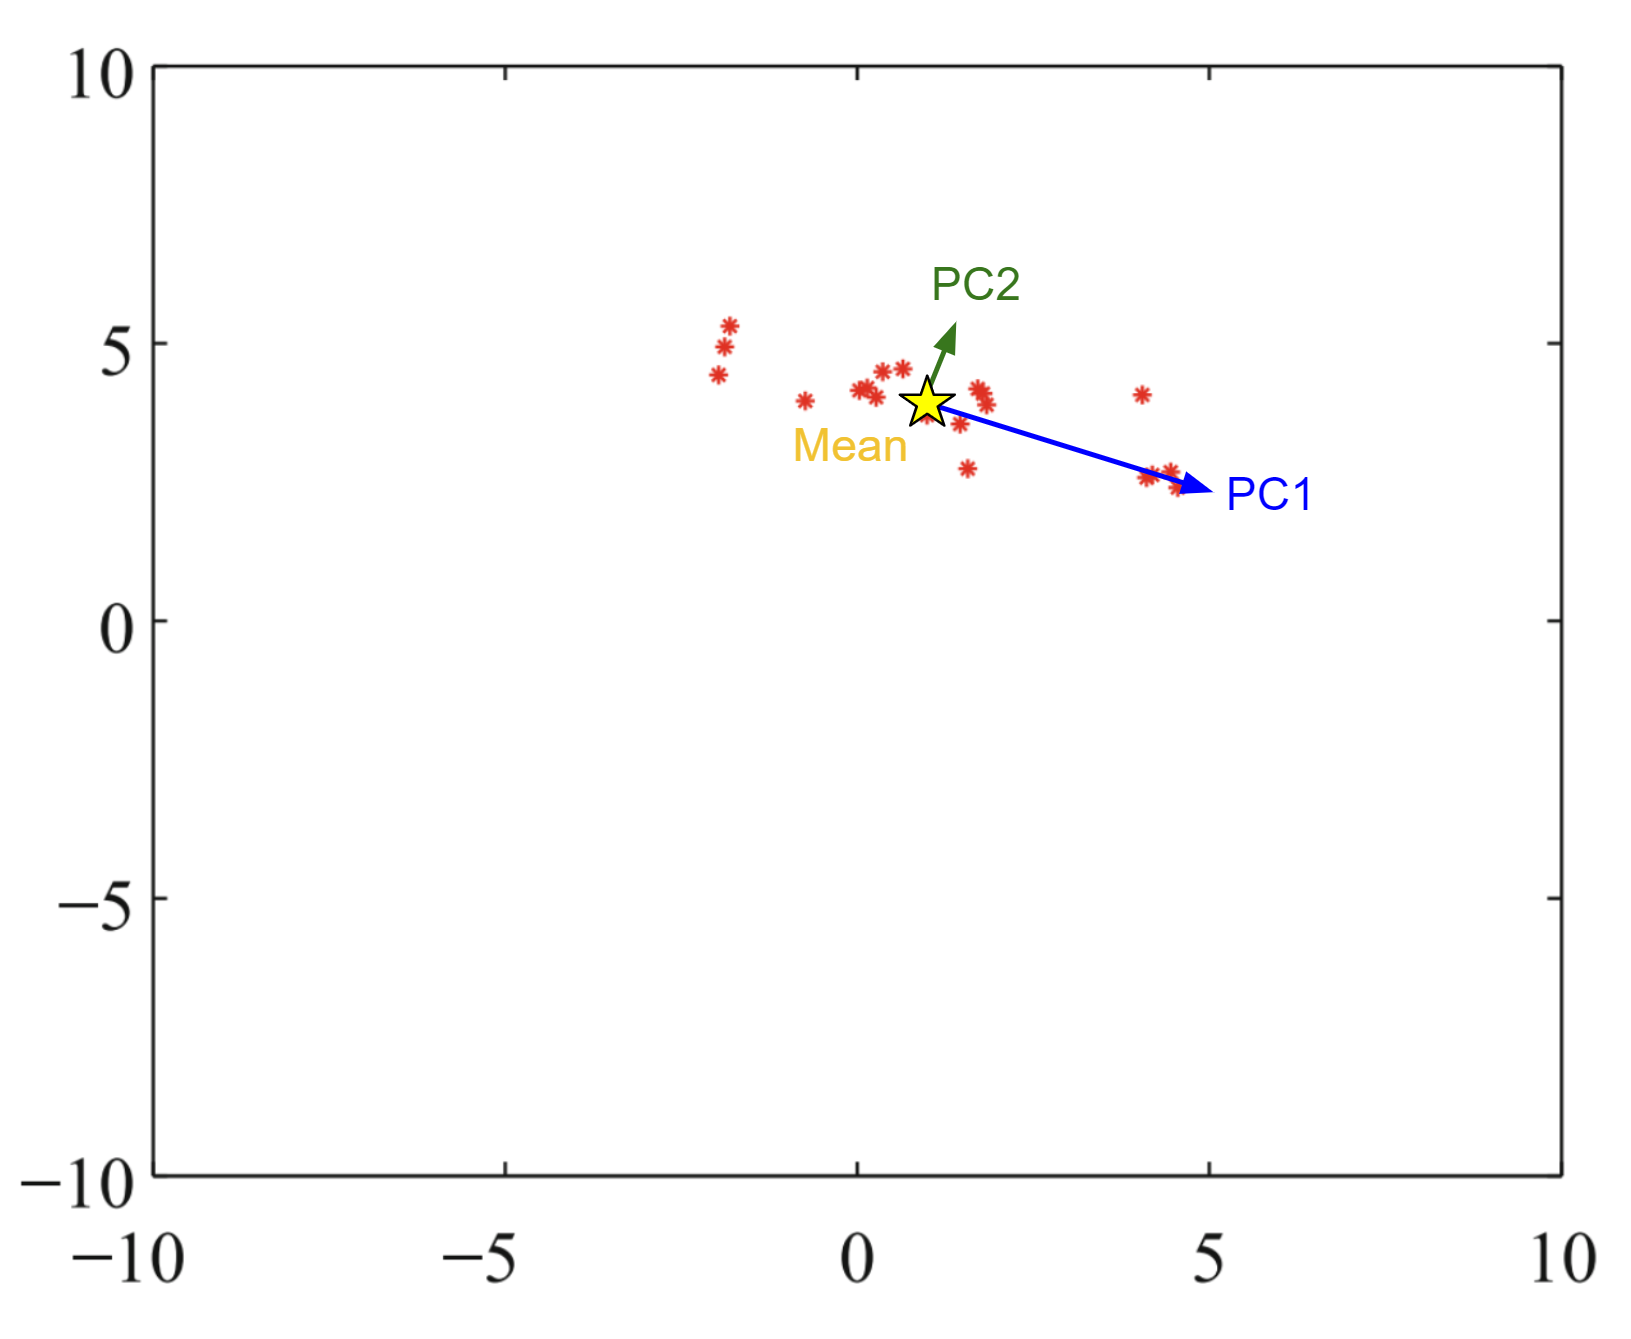
\includegraphics[scale=0.8]{HW9_1.PNG}
 
 
 \newpage
 
 \noindent\makebox[\linewidth]{\rule{\paperwidth}{0.4pt}}\newline
 
 \begin{center}
      \Large\textbf{Problem 2:} Take the wine dataset from the UC Irvine machine learning data repository at https://archive.ics.uci.edu/ml/datasets/Wine. \par
 \end{center}
 
 \textbf{Part A: | Plot the eigenvalues of the covariance matrix in sorted order. How many principal components should be used to represent this dataset? Why?}\newline
 
 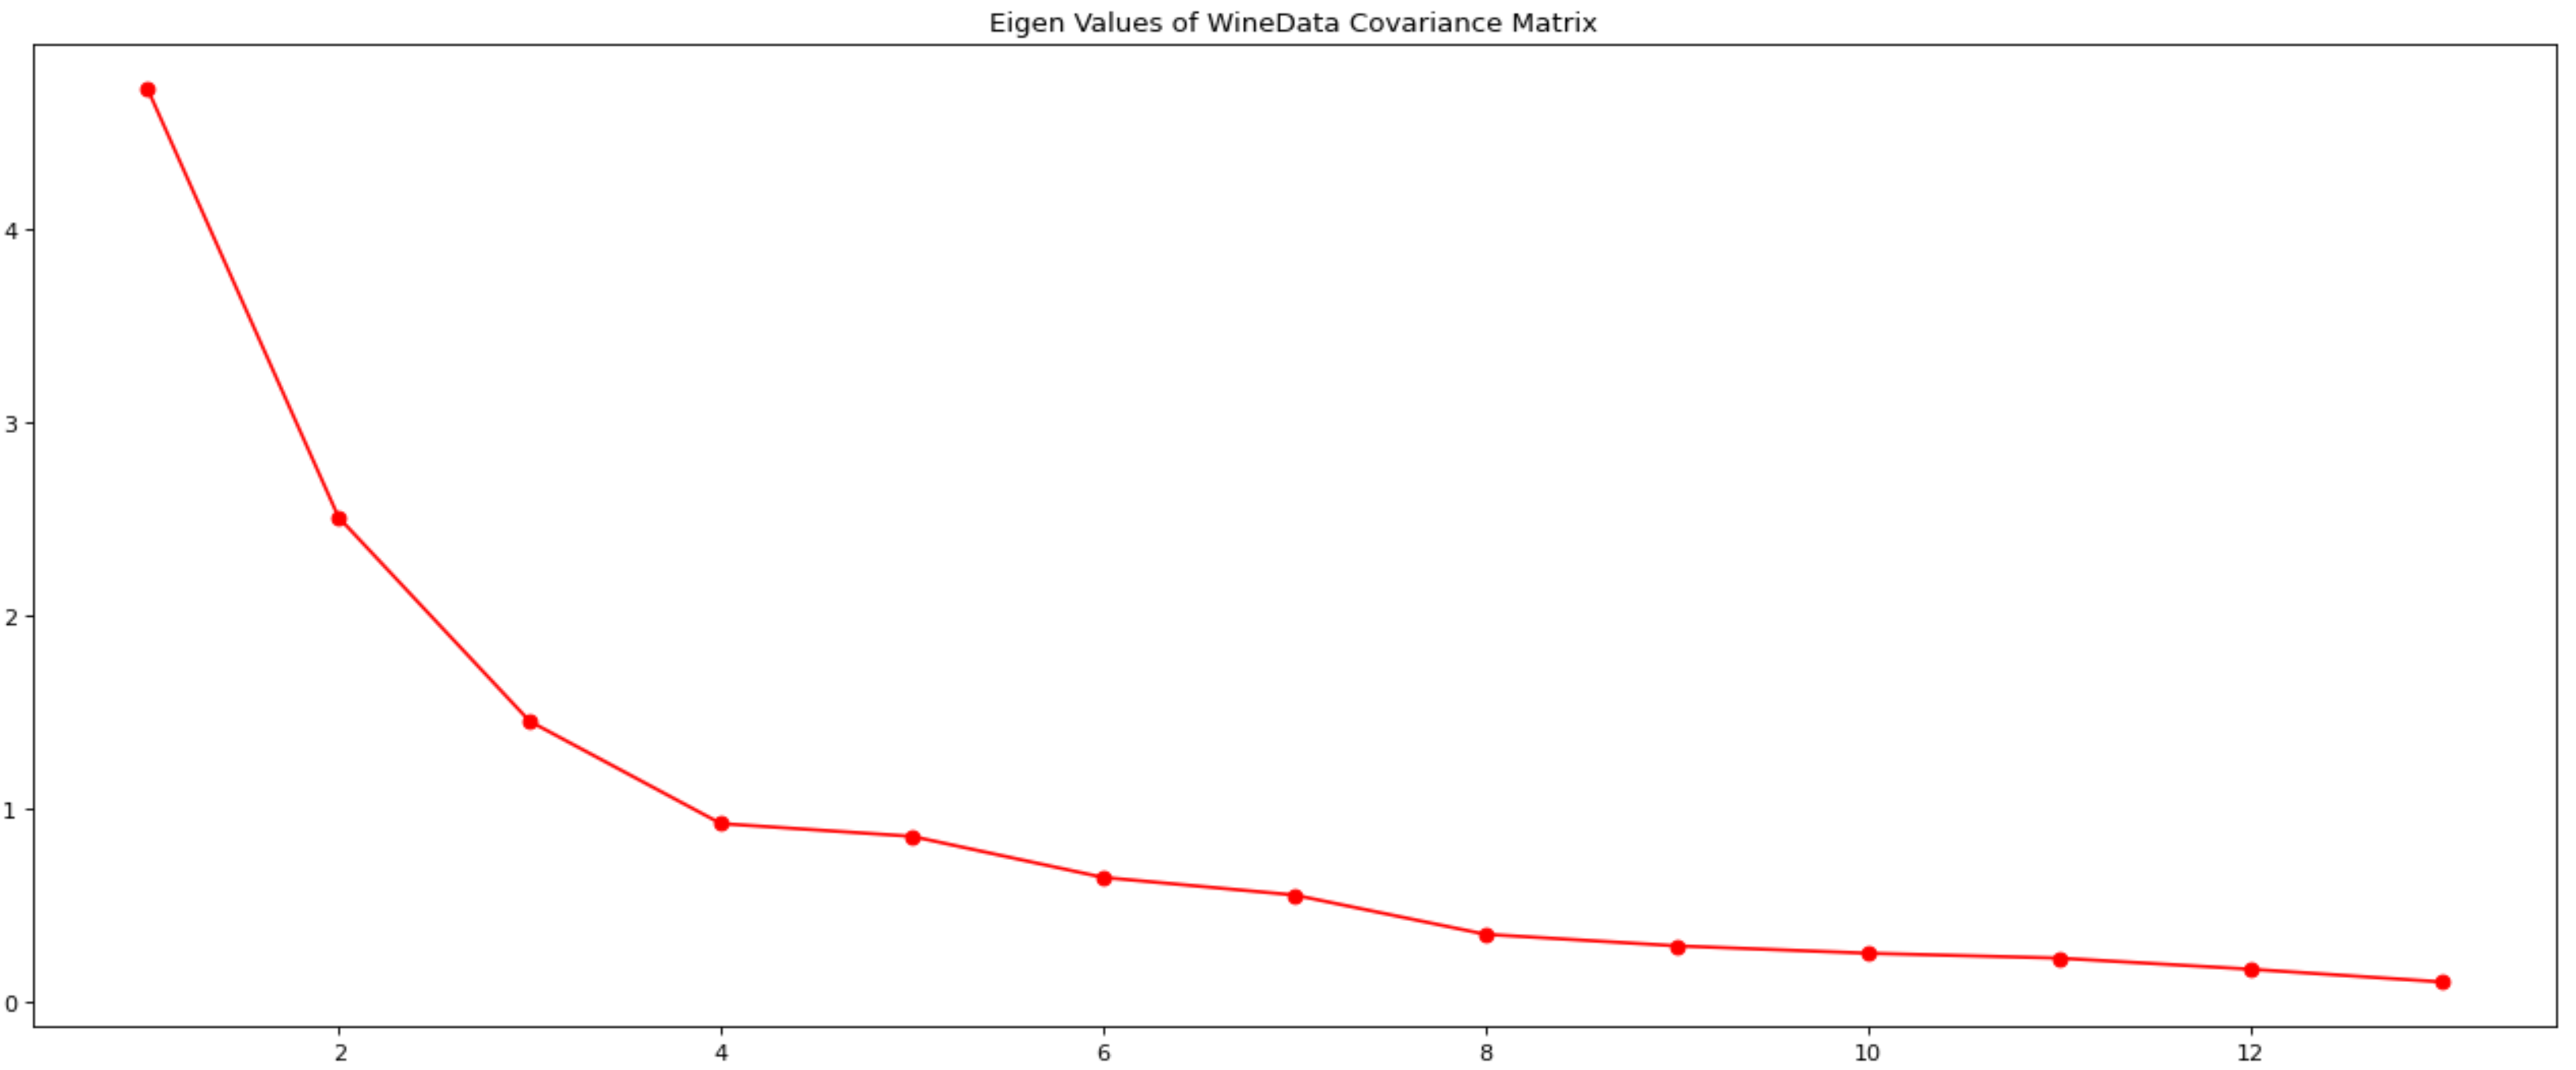
\includegraphics[scale=0.4]{HW9_2.PNG}\newline
 
 From viewing the first graph, we see that certain eigen values are much higher than others. We need not use all 13 principal components to represent our dataset accurately; in fact, using the 5 principal components which correspond to the 5 highest eigen values should be adequate. We find that the sum of the top 5 eigen values is more than 80\% of the sum of all the eigen values. Although the estimate isn't exact, it saves a lot of time and computation. Using 13 principal components would require immense resources and would be quite difficult to understand.
 
 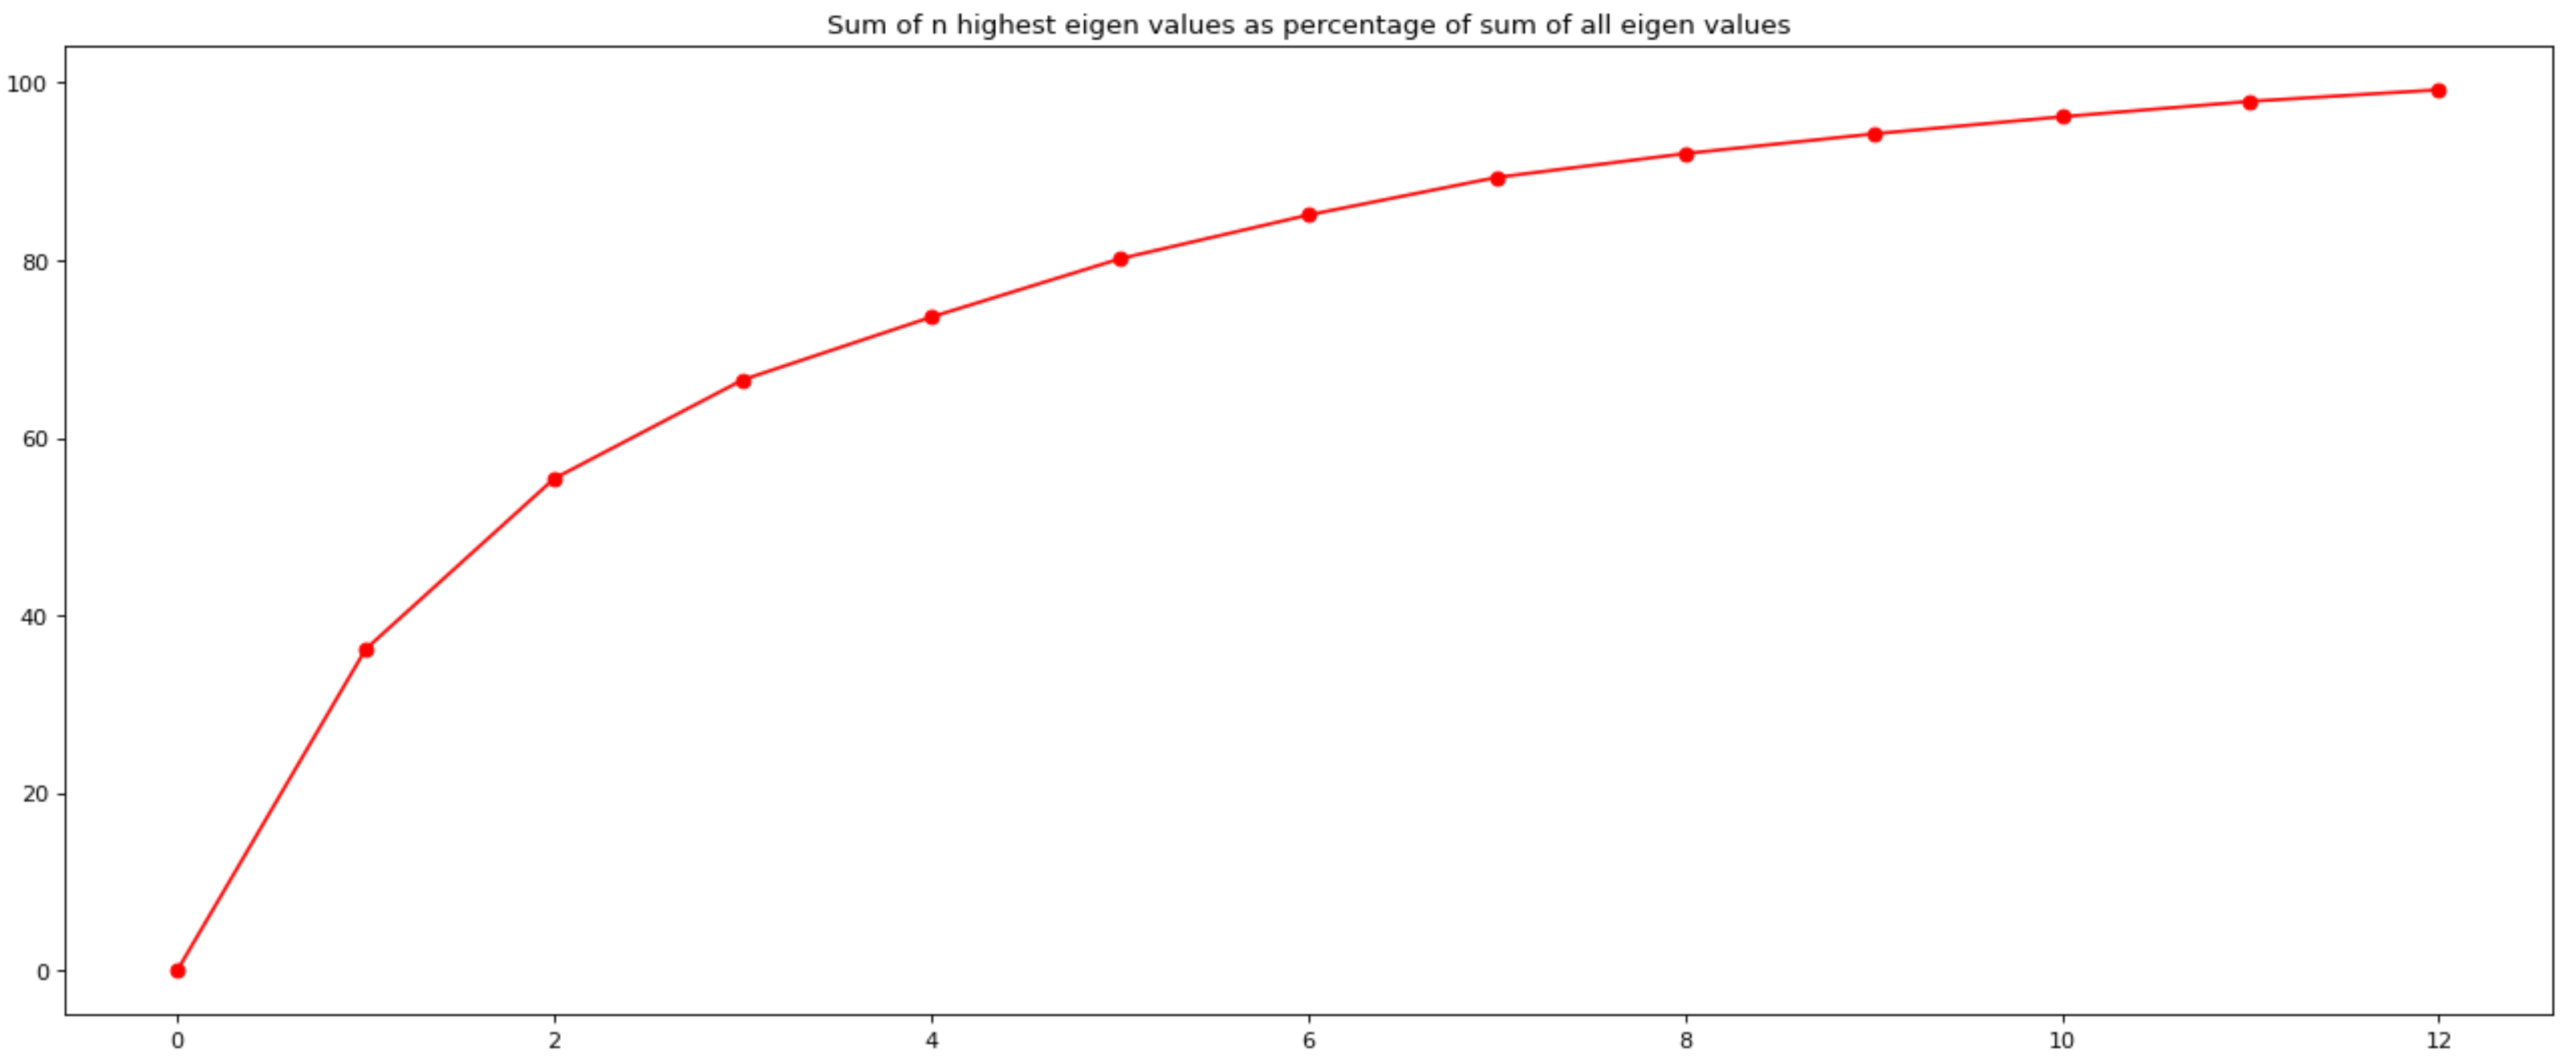
\includegraphics[scale=0.4]{HW9_3.PNG}\newline
 
 \newline
 
 \textbf{Part C: | Compute the first two principal components of this dataset, and project it onto those components. Now produce a scatter plot of this two dimensional dataset, where data items of class 1 are plotted as a ‘1’, class 2 as a ‘2’, and so on.}\newline
 
 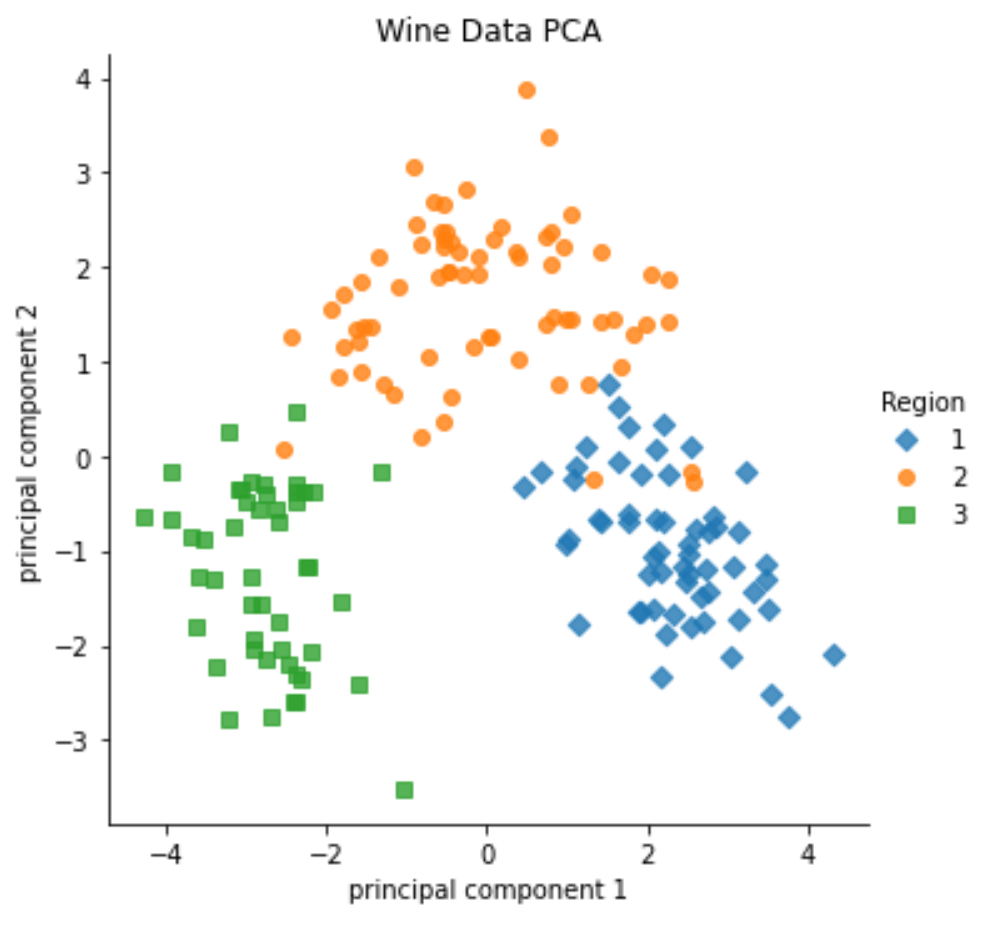
\includegraphics[scale=1]{HW9_4.PNG}\newline
 
 \newpage

 \begin{center}
      \Large\textbf{Problem 3:} Take the wheat kernel dataset from the UC Irvine machine learning data repository at http://archive.ics.uci.edu/ml/datasets/seeds. Compute the first two principal components of this dataset, and project it onto those components.
      \par
 \end{center}

 \textbf{Part A: | Produce a scatterplot of this projection. Do you see any interesting phenomena?}\newline
 
 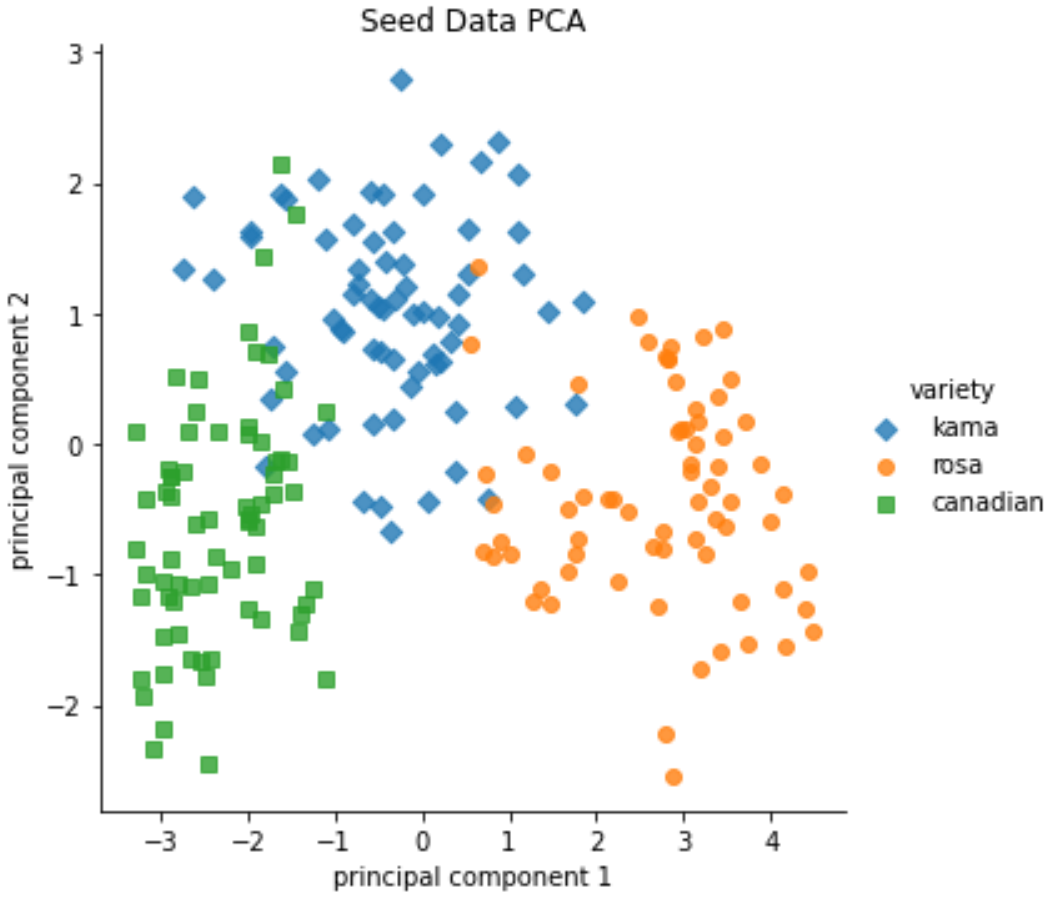
\includegraphics[scale=1]{HW9_5.PNG}\newline
 
 The most interesting phenomenon is that the different varieties of wheat occupy different "sectors" of the graph. Even though we only used two principal components, the data is classified quite well into discrete sections. Despite the classification, however, there doesn't appear to be all that much correlation between the two principal components; the data points show up as blobs instead of resembling a line or other relation. However, ignoring the variety, the data points appear to form an upside-down U-shape (an arch), indicating a weak but interesting correlation.\newline
 
 \textbf{Part B: | Plot the eigenvalues of the covariance matrix in sorted order. How many principal components should be used to represent this dataset? why?}\newline
 
 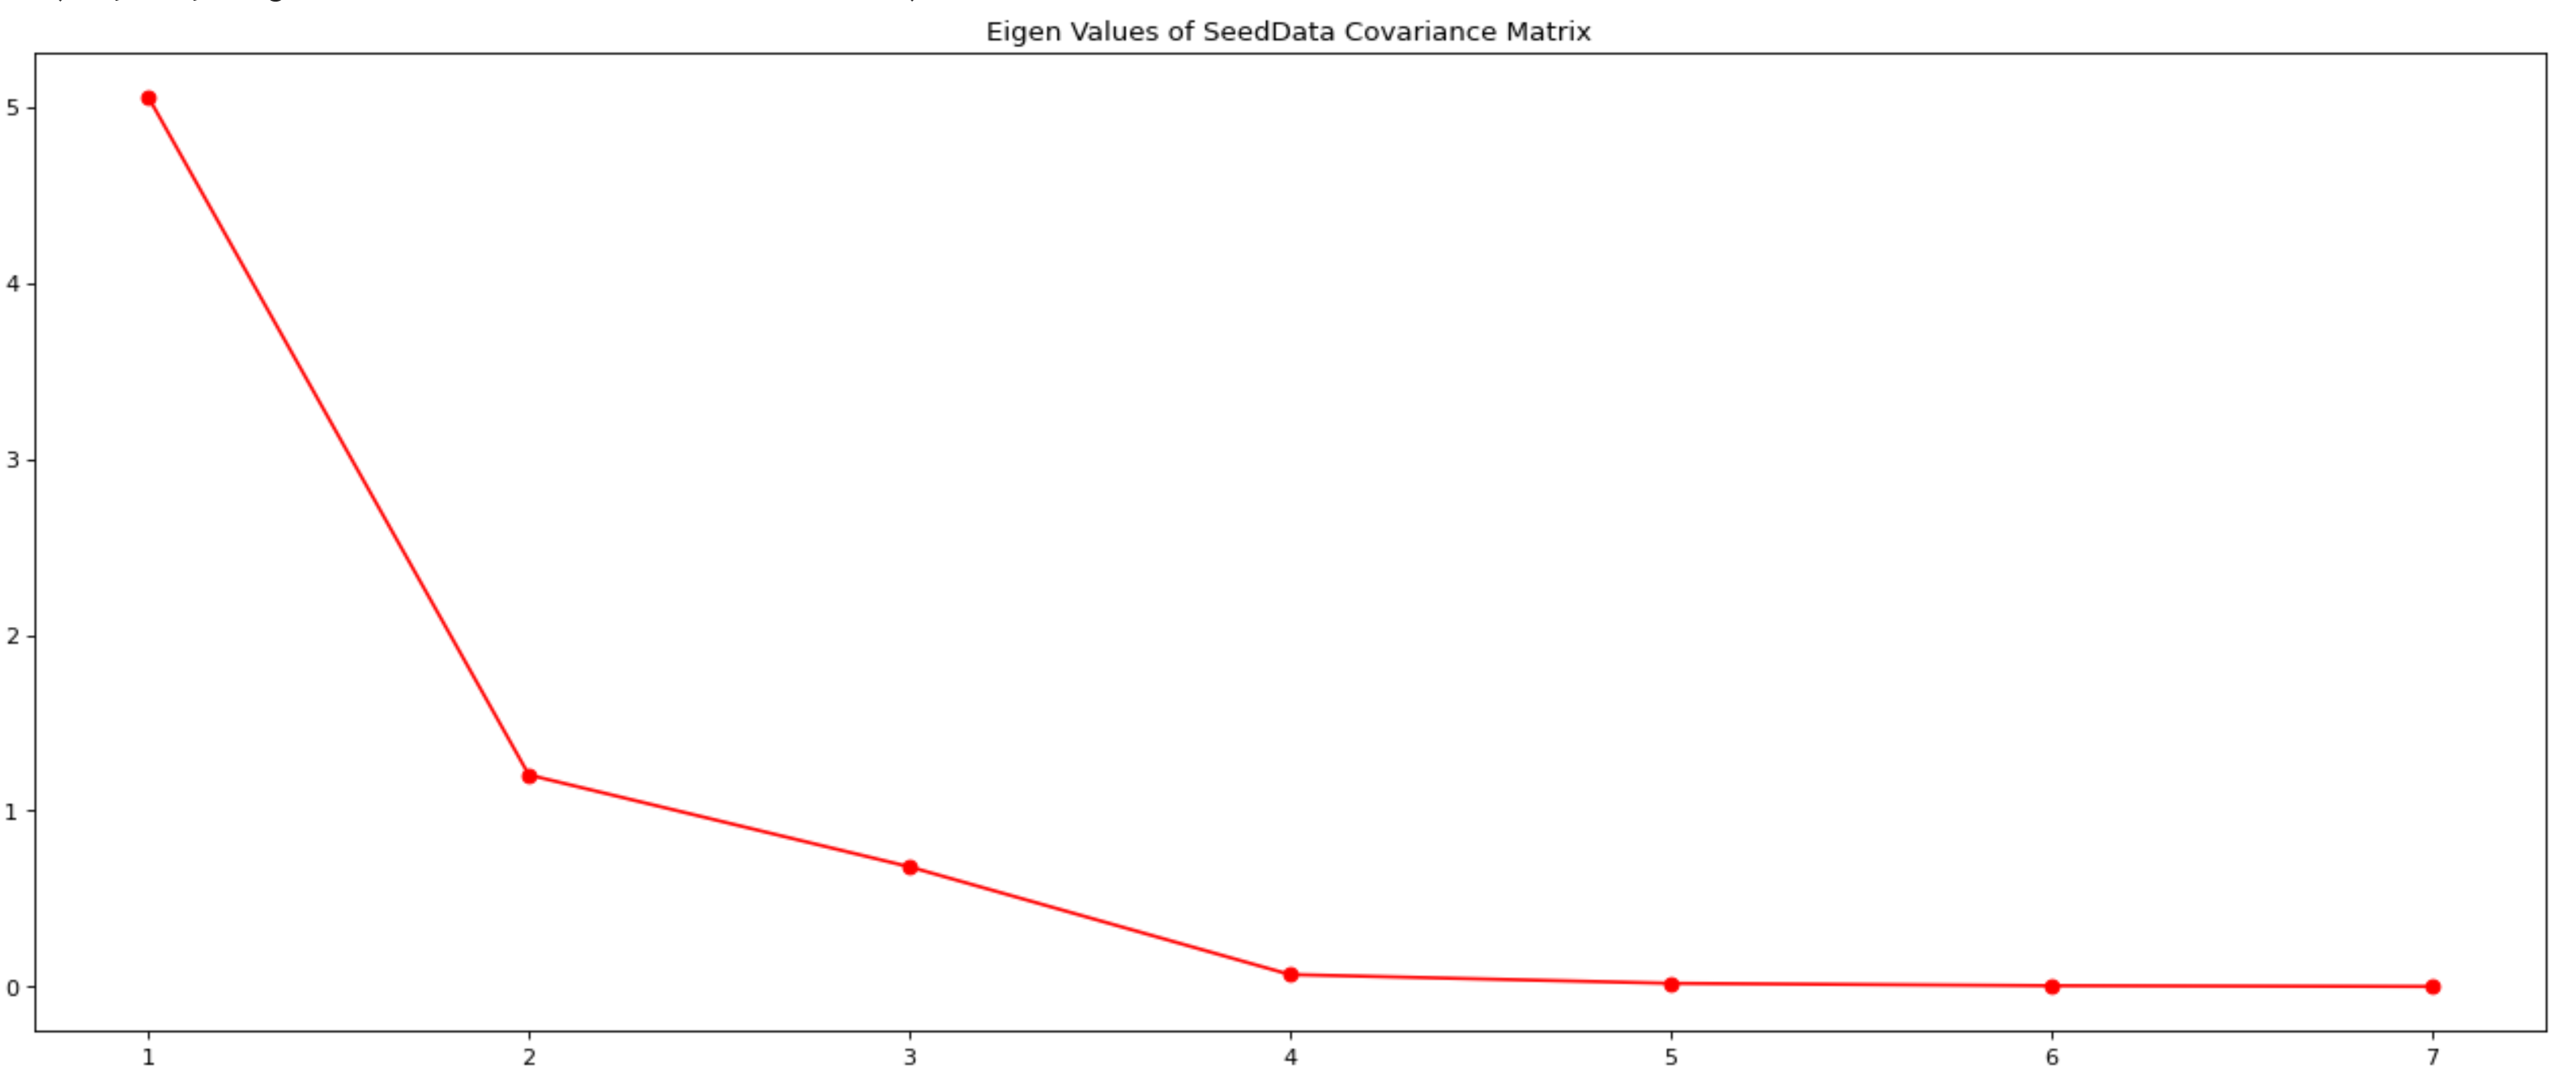
\includegraphics[scale=0.4]{HW9_6.PNG}\newline
 
 We should use only 3 of the 7 pricipal components to represent this dataset. The graph below shows that the sum of the 3 highest eigen values is around 99\% of the sum of all the eigen values. Using all 7 principal components would be a waste of resources, because our representation does not become much more accurate. The three principal components which correspond to the 3 highest eigen values carry more than enough information required to perform principal component analysis. We save computational resources and lower complexity without significantly affecting accuracy by using only 3 principal components. 
 
 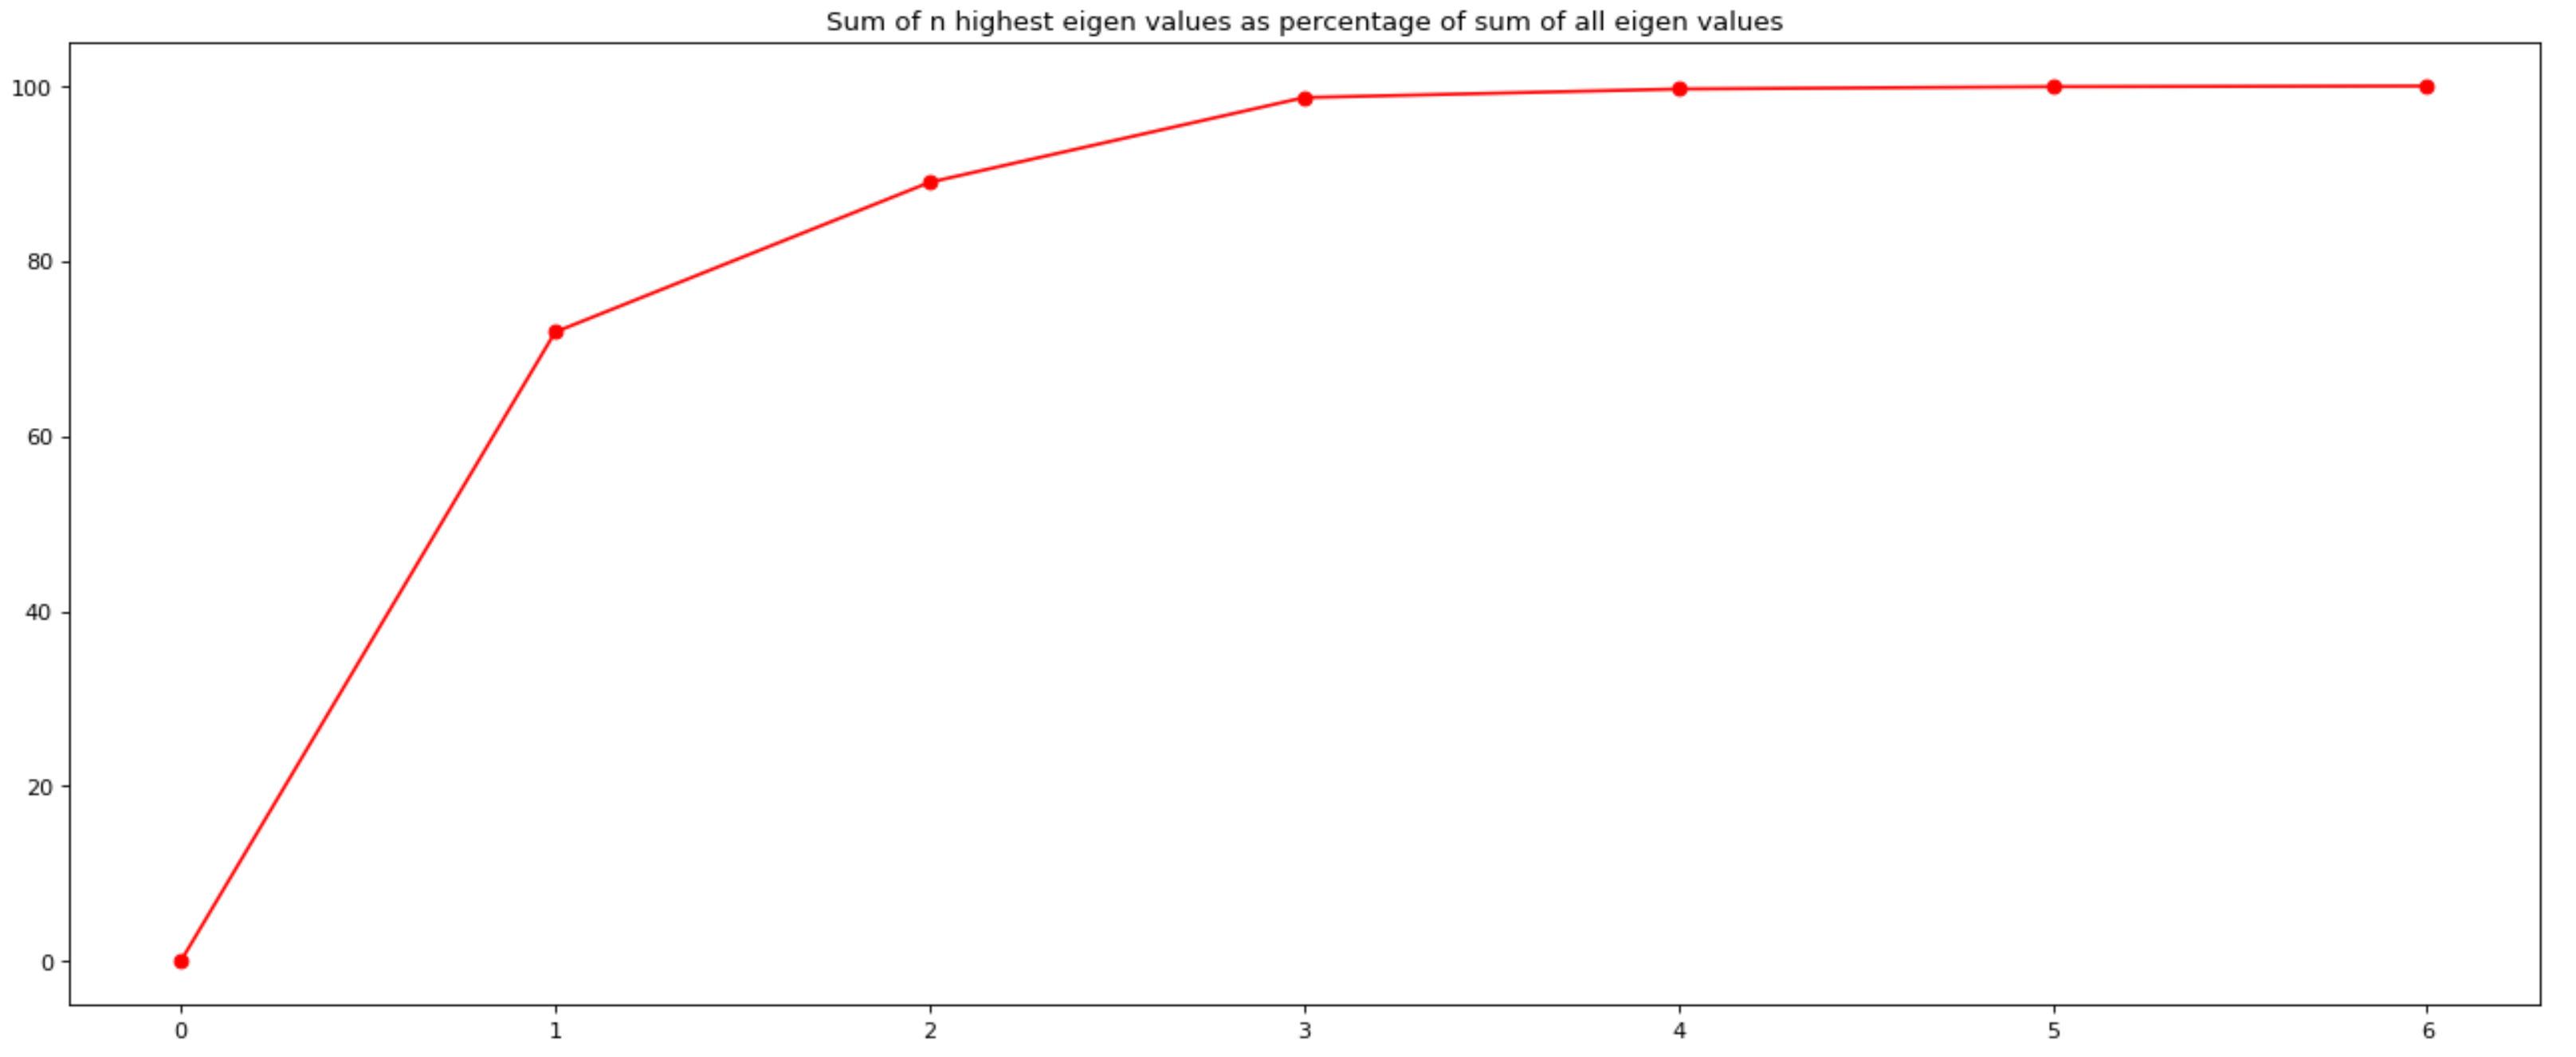
\includegraphics[scale=0.4]{HW9_7.PNG}\newline

 \newpage
 
 \begin{center}
      \Large\textbf{Problem 4:} Suppose you have a dataset $\{x\}=\{(x^{(1)}, x^{(2)})\}$ consisting of 2-dimensional vectors. You observe that $var(\{x^{(1)}\})=9$ and $var(\{x^{(2)}\})=4$ and also that $cov(\{(x^{(1)}, x^{(2)})\})=6$. \par
 \end{center}
 
 \textbf{Part A: |What is $Covmat(\{x\})$?}\newline
 
 We know that the covariance matrix is found by multiplying the transpose of a dataset with the dataset (represented as a matrix, of course). Using this fact, along with the fact that the covariance of a feature with itself is simply the variance, allows us to construct $Covmat(\{x\})$.
 
 \begin{bmatrix}
     9 & 6\\
     6 & 4
 \end{bmatrix}\newline
 
 \textbf{Part B: |Find the eigenvalues of $Covmat(\{x\})$.}\newline
 
 \[A = \begin{bmatrix}
     9 & 6\\
     6 & 4
 \end{bmatrix}
 \]
 
 \[|A-I\cdot\lambda| = 0\]
 
 \[|A-I\cdot\lambda| = 
 |
 \begin{bmatrix}
     9 & 6\\
     6 & 4
 \end{bmatrix} - 
 \begin{bmatrix}
     \lambda & 0\\
     0 & \lambda
 \end{bmatrix}
 |
 = 0
 \]
 
 \[
 |
 \begin{bmatrix}
     9 - \lambda & 6\\
     6 & 4 - \lambda
 \end{bmatrix}
 |
 = 0
 \]
 
 \[(9-\lambda)(4-\lambda)-36=0\]
 
 \[36-13\lambda+\lambda^2-36=0\]
 
 \[\lambda^2-13\lambda=0\]
 
 \[\lambda(\lambda-13)=0\]
 
 \[\lambda=\{0,13\}\]
 
 Final Answer: $0$ and $13$.\newline
 
 \newline
 
 \textbf{Part C: |What do the eigenvalues say about the shape of the blob of the dataset $\{x\}$?}\newline
 
 Because only one of the two eigenvalues is nonzero, we can conclude that the dataset is found along a line. The principal component coresponding to the eigenvalue of 13 contains all the "information" about the dataset. The entire dataset lies on one straight line, and only one principal component is required for analysis.
 
 \newpage
 
 \begin{center}
     \Large\textbf{Problem 5 (Correct Version):} Question too big to write ... \par
 \end{center}
 
 We must first create the matrix A with the given eigenvectors. We are using the first two eigenvectors: $u_1$ and $u_2$.
 
 \[A = 
 \begin{bmatrix}
     0.5 & 0.5 \\
     0.5 & -0.5 \\
     0.5 & -0.5 \\
     0.5 & 0.5 \\
 \end{bmatrix}
 \]
 
 We must then find $x_1 - mean(\{x\})$.
 
 \[x_1 - mean(\{x\})=
 \begin{bmatrix}
     2 \\
     2 \\
     4 \\
     6 \\
 \end{bmatrix}
 \]
 
 Finally, we can use the formula $\hat{x_1} = A^T[x_1 - mean(\{x\})]$ to find the coordinates of the projected point which represents $x_1$.
 
 \[\hat{x_1}=
 \begin{bmatrix}
     0.5 & 0.5 & 0.5 & 0.5 \\
     0.5 & -0.5 & -0.5 & 0.5 \\
 \end{bmatrix}
  \begin{bmatrix}
     2 \\
     2 \\
     4 \\
     6 \\
 \end{bmatrix}
 \]
 
 \[\hat{x_1}=
 \begin{bmatrix}
     7 \\
     1 \\
 \end{bmatrix}
 \]
 
 \newpage
 
 
 \begin{center}
     \Large\textbf{Problem 5:} Too big to write ... \par
 \end{center}
 
 \[\hat{x_i}=mean(\{x\})+\sum_{j=1}^{s}[{u_j}^T(x_i-mean(\{x\}))]u_j\]
 
 \[\hat{x_1}=
 \begin{bmatrix}
     1 \\
     1 \\
     1 \\
     1 \\
 \end{bmatrix}
 +\sum_{j=1}^{2}[{u_j}^T(x_1-mean(\{x\}))]u_j\]
 
 \[\hat{x_i}=
 \begin{bmatrix}
     1 \\
     1 \\
     1 \\
     1 \\
 \end{bmatrix}
 +[
 \begin{bmatrix}
     0.5 & 0.5 & 0.5 & 0.5 \\
 \end{bmatrix}
 \begin{bmatrix}
     2 \\
     2 \\
     4 \\
     6 \\
 \end{bmatrix}
 ]
 \begin{bmatrix}
     0.5 \\
     0.5 \\
     0.5 \\
     0.5 \\
 \end{bmatrix}
 +
 [
 \begin{bmatrix}
     0.5 & -0.5 & -0.5 & 0.5 \\
 \end{bmatrix}
 \begin{bmatrix}
     2 \\
     2 \\
     4 \\
     6 \\
 \end{bmatrix}
 ]
 \begin{bmatrix}
     0.5 \\
     -0.5 \\
     -0.5 \\
     0.5 \\
 \end{bmatrix}
 \]
 
 \[\hat{x_i}=
 \begin{bmatrix}
     1 \\
     1 \\
     1 \\
     1 \\
 \end{bmatrix}
 +[7]
 \begin{bmatrix}
     0.5 \\
     0.5 \\
     0.5 \\
     0.5 \\
 \end{bmatrix}
 +
 [1]
 \begin{bmatrix}
     0.5 \\
     -0.5 \\
     -0.5 \\
     0.5 \\
 \end{bmatrix}
 \]
 
 \[\hat{x_i}=
 \begin{bmatrix}
     1 \\
     1 \\
     1 \\
     1 \\
 \end{bmatrix}
 +
 \begin{bmatrix}
     3.5 \\
     3.5 \\
     3.5 \\
     3.5 \\
 \end{bmatrix}
 +
 \begin{bmatrix}
     0.5 \\
     -0.5 \\
     -0.5 \\
     0.5 \\
 \end{bmatrix}
 \]
 
 \[\hat{x_i}=
 \begin{bmatrix}
     5 \\
     4 \\
     4 \\
     5 \\
 \end{bmatrix}
 \]
 
 \newpage
 
 \end{document}

